\documentclass[border=10pt]{standalone}
\usepackage{tikz}
\usepackage{amsmath,amssymb}
\usetikzlibrary{arrows.meta,positioning,calc,fit,backgrounds}

% Pre-define colors
\definecolor{swinblue}{RGB}{70,130,200}
\definecolor{swinbluefill}{RGB}{220,235,250}
\definecolor{tikorange}{RGB}{220,150,50}
\definecolor{tikorgfill}{RGB}{255,240,220}
\definecolor{projgreen}{RGB}{60,150,80}
\definecolor{projgrfill}{RGB}{220,245,225}
\definecolor{msecolor}{RGB}{200,70,70}
\definecolor{msefill}{RGB}{255,225,225}
\definecolor{combpurple}{RGB}{130,70,170}
\definecolor{combfill}{RGB}{240,225,255}
\definecolor{clsviolet}{RGB}{150,80,180}
\definecolor{clsfill}{RGB}{245,230,255}

\begin{document}
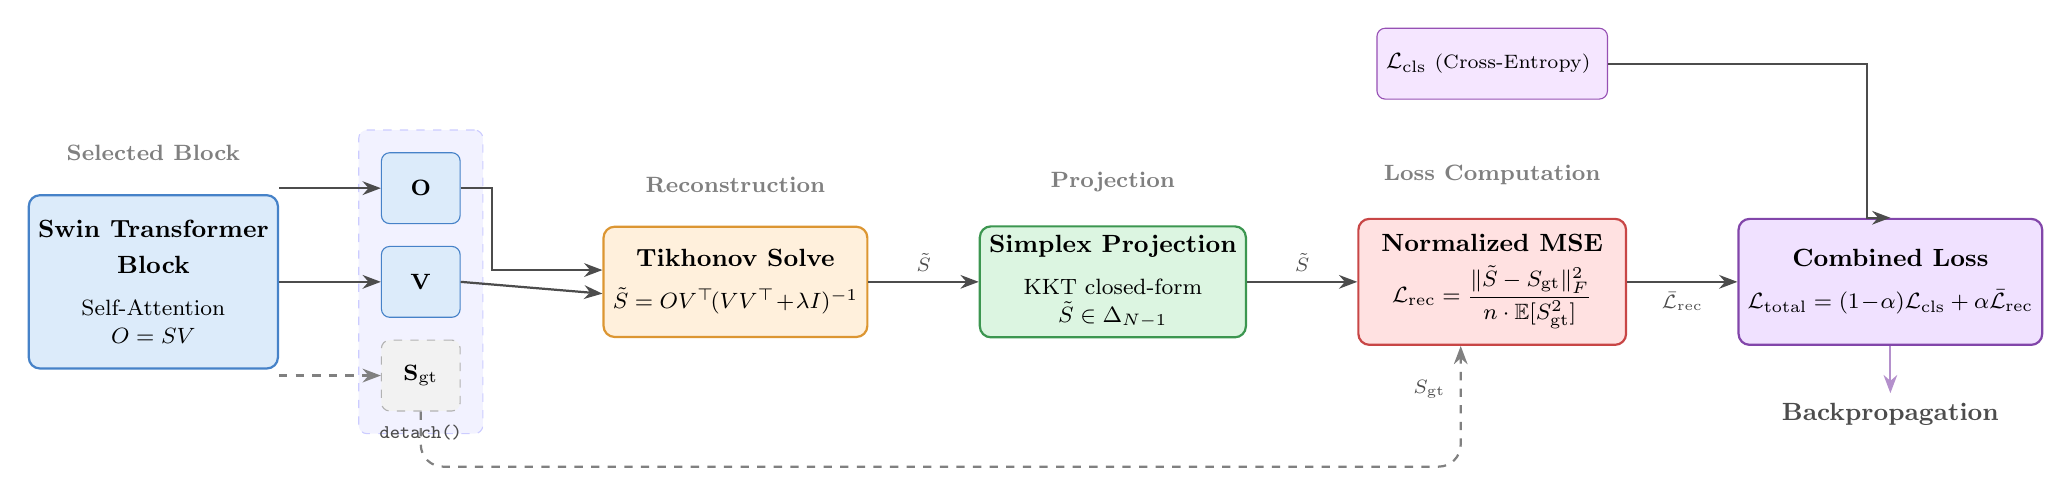
\begin{tikzpicture}[
    >=Stealth,
    node distance=1.2cm and 1.6cm,
    every node/.style={font=\small},
    arrow/.style={->, line width=0.8pt, color=black!70},
    dasharrow/.style={->, line width=0.8pt, dashed, color=black!50},
    lbl/.style={font=\scriptsize, color=black!70},
]

% === Swin Transformer Block ===
\node[rectangle, rounded corners=4pt, draw=swinblue, fill=swinbluefill,
      minimum width=2.8cm, minimum height=2.2cm, align=center, line width=0.8pt]
    (swin) {
    \textbf{Swin Transformer}\\[2pt]\textbf{Block}\\[4pt]
    {\footnotesize Self-Attention}\\[-1pt]
    {\footnotesize $O = SV$}
};

% === Output nodes from Swin block ===
\node[right=1.8cm of swin.north east, anchor=north, yshift=0.2cm] (O) {};
\node[right=1.8cm of swin.east, anchor=center] (V) {};
\node[right=1.8cm of swin.south east, anchor=south, yshift=-0.2cm] (Sgt) {};

% Small boxes for O, V, S_gt
\node[rectangle, rounded corners=3pt, draw=swinblue, fill=swinbluefill,
      minimum width=1.0cm, minimum height=0.9cm, align=center, font=\footnotesize]
    at (O) (Obox) {$\mathbf{O}$};
\node[rectangle, rounded corners=3pt, draw=swinblue, fill=swinbluefill,
      minimum width=1.0cm, minimum height=0.9cm, align=center, font=\footnotesize]
    at (V) (Vbox) {$\mathbf{V}$};
\node[rectangle, rounded corners=3pt, draw=gray!60, fill=gray!10, dashed,
      minimum width=1.0cm, minimum height=0.9cm, align=center, font=\footnotesize]
    at (Sgt) (Sgtbox) {$\mathbf{S}_{\text{gt}}$};

\draw[arrow] (swin.east |- Obox) -- (Obox.west);
\draw[arrow] (swin.east |- Vbox) -- (Vbox.west);
\draw[dasharrow] (swin.east |- Sgtbox) -- (Sgtbox.west);

% detach label
\node[lbl, below=0.05cm of Sgtbox] {\texttt{detach()}};

% === Tikhonov Solve ===
\node[rectangle, rounded corners=4pt, draw=tikorange, fill=tikorgfill,
      minimum height=1.4cm, minimum width=3.2cm, align=center, line width=0.8pt,
      right=1.8cm of Vbox]
    (tik) {
    \textbf{Tikhonov Solve}\\[4pt]
    {\footnotesize $\tilde{S} = OV^\top\!(VV^\top\!+\!\lambda I)^{-1}$}
};

\draw[arrow] (Obox.east) -- ++(0.4,0) |- ([yshift=0.15cm]tik.west);
\draw[arrow] (Vbox.east) -- ([yshift=-0.15cm]tik.west);

% === Simplex Projection ===
\node[rectangle, rounded corners=4pt, draw=projgreen, fill=projgrfill,
      minimum height=1.4cm, minimum width=2.8cm, align=center, line width=0.8pt,
      right=1.4cm of tik]
    (proj) {
    \textbf{Simplex Projection}\\[4pt]
    {\footnotesize KKT closed-form}\\[-1pt]
    {\footnotesize $\tilde{S} \in \Delta_{N-1}$}
};

\draw[arrow] (tik.east) -- node[above, lbl] {$\tilde{S}$} (proj.west);

% === Normalized MSE ===
\node[rectangle, rounded corners=4pt, draw=msecolor, fill=msefill,
      minimum height=1.6cm, minimum width=3.4cm, align=center, line width=0.8pt,
      right=1.4cm of proj]
    (mse) {
    \textbf{Normalized MSE}\\[4pt]
    {\footnotesize $\mathcal{L}_{\text{rec}} = \dfrac{\|\tilde{S} - S_{\text{gt}}\|_F^2}{n \cdot \mathbb{E}[S_{\text{gt}}^2]}$}
};

\draw[arrow] (proj.east) -- node[above, lbl] {$\tilde{S}$} (mse.west);

% S_gt dashed arrow to MSE (curved below)
\draw[dasharrow, rounded corners=8pt]
    (Sgtbox.south) -- ++(0,-0.7) -| ([xshift=-0.4cm]mse.south);
\node[lbl] at ([yshift=-0.55cm, xshift=-0.8cm]mse.south) {$S_{\text{gt}}$};

% === Classification Loss (from top) ===
\node[rectangle, rounded corners=3pt, draw=clsviolet, fill=clsfill,
      minimum width=2.2cm, minimum height=0.9cm, align=center, font=\footnotesize,
      above=1.5cm of mse]
    (cls) {
    $\mathcal{L}_{\text{cls}}$ {\scriptsize (Cross-Entropy)}
};

% === Combined Loss ===
\node[rectangle, rounded corners=4pt, draw=combpurple, fill=combfill,
      minimum height=1.6cm, minimum width=3.2cm, align=center, line width=0.8pt,
      right=1.4cm of mse]
    (total) {
    \textbf{Combined Loss}\\[4pt]
    {\footnotesize $\mathcal{L}_{\text{total}} = (1\!-\!\alpha)\mathcal{L}_{\text{cls}} + \alpha\bar{\mathcal{L}}_{\text{rec}}$}
};

\draw[arrow] (mse.east) -- node[below, lbl] {$\bar{\mathcal{L}}_{\text{rec}}$} (total.west);
\draw[arrow] (cls.east) -| ([xshift=-0.3cm]total.north) -- (total.north);

% === Backprop arrow ===
\node[lbl, below=0.6cm of total, font=\small\bfseries] (bp) {Backpropagation};
\draw[->, line width=0.8pt, color=combpurple!60] (total.south) -- (bp.north);

% === Background for intermediate outputs ===
\begin{scope}[on background layer]
    \node[fit=(Obox)(Vbox)(Sgtbox), inner sep=8pt, fill=blue!5,
          rounded corners=3pt, draw=blue!20, dashed] {};
\end{scope}

% === Stage titles ===
\node[above=0.3cm of swin.north, font=\footnotesize\bfseries, color=black!50]
    {Selected Block};
\node[above=0.3cm of tik.north, font=\footnotesize\bfseries, color=black!50]
    {Reconstruction};
\node[above=0.3cm of proj.north, font=\footnotesize\bfseries, color=black!50]
    {Projection};
\node[above=0.3cm of mse.north, font=\footnotesize\bfseries, color=black!50]
    {Loss Computation};

\end{tikzpicture}
\end{document}
